\documentclass{article}

\usepackage[utf8]{inputenc}
\usepackage[T1]{fontenc}
\usepackage{geometry}
\usepackage{graphicx}   %ALLOWS INSERTING IMAGES (AND MAYBE SOME MORE STUFF) %
\usepackage{caption}
\usepackage{subcaption} %ALLOWS CAPTIONS FOR SUBFIGURES%
\usepackage{verbatim} % ALLOWS MULTILINE COMMENTS WITH \begin{comment} AND \end{comment} %
\usepackage{amsmath,amssymb} % PERMETTE L'USO DI SIMBOLI MATEMATICI "AVANZATI" COME 'MINORE O UGUALE' E ALTRI %
\usepackage{amstext}
\usepackage{enumitem} %PERMETTE L'USO DI ELENCHI NUMERATI
\usepackage[section]{placeins}

\geometry{a4paper}
                        %Una riga vuota tra due scritte spazia di una riga anche sul pdf. Andare a capo una volta non provoca nulla nel pdf%
\usepackage[italian,english]{babel}
%\usepackage[french, italian]{babel} non funzione per motivi a me ignoti
\frenchspacing 

%%%  INTESTAZIONE  %%%

\title{Relazione dell'esperimento di misura della velocità della luce}
\author{Lorenzo Ramella, Alessandro Matteo Rossi, Marco Tambini}
\date{\today}


%%%  INIZIO DOCUMENTO  %%%

\begin{document}
\maketitle

%%%  ABSTRACT  %%%
\begingroup
\selectlanguage{english}
\begin{abstract}
    \centering
L’esperimento si propone di misurare la velocità delle luce usando il metodo di Focault. Dopo l'analisi di un totale di 110 misure (di cui una rigettata), provenienti 
da due esperienze laboratoriali diverse, abbiamo ottenuto un valore per la velocità della luce pari a $c_{BEST}=2,982\cdot10^8 \pm 8,6\cdot 10^6 m/s$, compatibile
entro una $\sigma$ con il valore vero $c_{vero}=2,998\cdot10^8 m/s$.
\end{abstract}
\endgroup

%%%  INDICE  %%%%

\selectlanguage{italian}
\tableofcontents
\newpage

%%%  INTRODUZIONE TEORICA  %%%

\section{Introduzione teorica}
Il metodo di Focault per la misura della velocità della luce consiste nell'uso di uno specchio rotante, che riflette la luce emessa da una sorgente su di uno specchio 
concavo. 

\begin{figure}[h!]
    \centering
    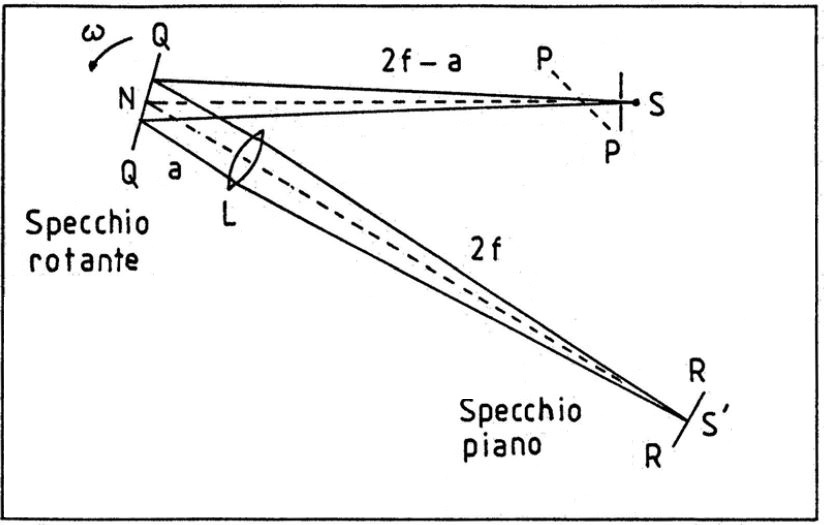
\includegraphics[width=0.5\linewidth]{App_Focault.JPG}
    \caption{Apparato di Focault BISOGNA CAMBIARE LA DICITURA SPECCHIO PIANO}
    \label{App_Focault}
\end{figure}

Una sorgente luminosa $S$ emette una luce che diaframmata da una lente $L_1$ attraversa una lastra semiriflettente angolata di 45° rispetto alla 
direzione del fascio. Una lente $L_2$ focalizza il fascio nel punto $S'$ sullo specchio concavo, dopo essere stata deflessa dallo specchio rotante. La luce riflessa 
dallo specchio concavo viene deflessa nuovamente dallo specchio rotante, che nel frattempo ha ruotato di un angolo 

\begin{equation}
\alpha = \omega \frac{2D}{c}
\end{equation}

dove $\omega$ è la velocità angolare dello specchio e $D$ è la distanza tra lo specchio rotante e lo specchio concavo.

Il fascio luminoso di ritorno sulla lente $L_2$ viene focalizzato come se provenisse da una sorgente $S''$ spostata da $S'$ di una quantità 

\begin{equation}
\Delta = 2 \alpha D
\label{DELTA}
\end{equation}

Sapendo che il fattore di amplificazione $G$ della lente $L_2$ è esprimibile come:

\begin{equation}
G=\frac{b}{D+a}
\label{G}
\end{equation}

dove $b$ è la distanza tra $L_2$ e la sorgente luminosa e $a$  la distanza tra $L_2$ e lo specchio rotante. Lo spostamento laterale $\delta$ dell'immagine si ottiene quindi
combinando le equazioni (\ref{DELTA}) e (\ref{G})
\begin{equation}
\delta = G\Delta =\frac{2\alpha b D}{D + a}=\frac{4 D^2 b \omega}{c(D+a)}
\label{delta}
\end{equation}

È possibile ricavare $b$ dalla legge dei punti coniugati. Sapendo che:

\begin{equation}
\frac{1}{b}+\frac{1}{D+a}=\frac{1}{f_2}
\label{punticoniug}
\end{equation}

Si deduce che:

\begin{equation}
b=\frac{f_2(D+a)}{D+a-f_2}
\end{equation}

E quindi, conoscendo l'espressione di $\delta$ dalla equazione (\ref{delta}), in cui compare $c$, e avendo ricavato l'unica variabile incognita $b$ dall'equazione
(\ref{punticoniug}), si ottiene:

\begin{equation}
c = \frac{4f_2D^2(\omega-\omega_0)}{[(D+a-f_2)\Delta\delta]}
\label{c_equation}
\end{equation}

dove $\omega_0$ è la velocità angolare iniziale e $\Delta\delta = \omega - \omega_0$ è lo spostamento dell'immagine della sorgente luminosa.

\begin{figure}[h]
    \centering
        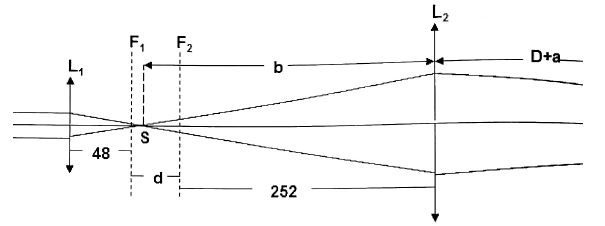
\includegraphics[width=0.6\linewidth]{IntroTeorica1.JPG}
    \caption{Schema apparato - intorno del beam-splitter}
\end{figure}

%%%  PROGETTAZIONE DELL'ESPERIMENTO  %%%

\newpage

\section{Progettazione dell'esperimento}

\begin{figure}[h] 
    \centering
    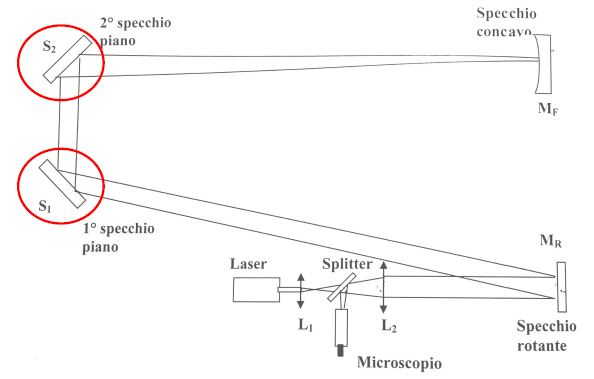
\includegraphics[width=0.6\linewidth]{Progettazione1.JPG}
    \caption{Schema dell'apparato di laboratorio}
    \label{schema_apparato}
\end{figure}

Il banco ottico di laboratorio era composto da un binario magnetico dove erano già presenti una sorgente luminosa e uno specchio rotante fissati magneticamente,
e un sistema di specchi ancorato saldamente al tavolo mediante morse. Sul binario magnetico era possibile aggiungere lenti, squadrette e lamine polaroid anch'esse con base
magnetica. Tutto l'apparato è schematicamente rappresentato in Figura \ref{schema_apparato}.

Prima di cominciare le misure di $c$ è necessario assicurarsi che gli elementi del banco ottico siano correttamente posizionati.

\vspace{3mm}

Per fare ciò abbiamo in principio misurato la lunghezza del cammino ottico $D$ del raggio luminoso dallo specchio rotante allo specchio concavo, raccogliendo 
4 misure per le distanze tra specchio rotante e specchio 1 $d_{rot,1}$, tra specchio 1 e specchio 2 $d_{1,2}$ e tra specchio 2 e specchio concavo $d_{2,conc}$, per poi 
ottenere tramite una somma delle loro medie aritmetiche il valore di $D$, con incertezza $\sigma D \approx 0,01 m = \sigma d$). Gli strumenti utilizzati in questa fase sono
stati due rotelle metriche di portata $15m$ e $3m$ entrambe sensibili al centimetro.

\vspace{3mm}

La sorgente luminosa coerente è un laser di potenza $0,35W$ che nonostante la bassa potenza ha richiesto l'utilizzo di una coppia di lamine polaroid per evitare danni agli
occhi; sono state apposte magneticamente sul binario subito dopo il laser.
Per permette alla luce di percorrere il sistema di specchi che va dallo specchio rotante, allo specchio $S_1$, quindi allo specchio $S_2$ e infine allo specchio concavo 
ci siamo inizialmente accertati che la luce incidesse sul centro dello specchio rotante, posizionando una squadretta forata con base magnetica sul binario.
Confermata la centratura del laser con lo specchio rotante, abbiamo quindi posto una prima lente $L_1$ a $70 mm$ seguendo la scala graduata con la sensibilità del 
millimetro presente sul binario per poter fare convergere la luce proveniente "dall'infinito" nel suo fuoco, che il produttore 
della lente dichiara essere a una distanza $f_1 = 0,048 m$. Abbiamo provveduto a regolare la posizione della lente per continuare ad avere il raggio centrato nel foro
della squadretta (e pertanto nel centro dello specchio rotante). A una distanza di $180mm$ dall'inizio della scala graduata abbiamo posizionato il beam-splitter, un elemento dotato di uno
specchio semiriflettente orientabile rispetto alla luce incidente, che permette di trasmettere la luce in arrivo alla lente $L_2$, e di riflettere quella in arrivo da 
$L_2$ verso l'alto, dove posizioneremo il microscopio, se angolato di $45^\circ$. La lente $L_2$, con focale dichiarata dal produttore di $f_2=0,252m$, è stata da noi 
apposta a circa $b = 370mm$ della scala graduata per ottenere un puntino sullo specchio concavo. 

\vspace{3mm}

Ultimato il posizionamento delle lenti, abbiamo agito sulla cinghia dello specchio rotante per permettere al raggio proveniente da $L_2$ di raggiungere la parte riflettente 
dello specchio e quindi subire una riflessione verso il centro (approssimativamente) di $S_1$.
Fatto questo abbiamo regolato l'inclinazione di $S_1$ per riflettere il raggio proveniente dallo specchio rotante approssimativamente nel centro di $S_2$, attraverso due
viti micrometriche poste dietro lo specchio. Abbiamo ripetuto quest'ultima manovra per portare il raggio dal centro di $S_2$ al centro dello specchio concavo.

Specifichiamo che a causa della complessità della misura della focale di una lente le focali e le posizioni corrette per lenti e beam-splitter vengono fornite dai 
docenti, e le consideriamo affette da un'incertezza trascurabile.

\vspace{3mm}

Raggiunta la condizione di raggio che percorre tutta la lunghezza $D$, era necessario agire nuovamente sulle viti micrometriche degli specchi per fare tornare il raggio
luminoso indietro fino al beam-splitter ripercorrendo il suo cammino di andata. È stato utile utilizzare un foglio di carta millimetrata da posizionare
a mezz'aria dove supponevamo che i raggi passassero, per verificare, spostando il foglio verso lo "specchio di destinazione", che i raggi coincidessero e che il puntino luminoso
del raggio di andata non si discostasse da quello del raggio di ritorno.

\vspace{3mm}

Verificato che il raggio di ritorno incidesse nel foro superiore del beam splitter, abbiamo inserito e messo a fuoco il microscopio (regolando l'altezza di fissaggio) nel
foro superiore del beam-splitter. Il microscopio è utile per osservare il raggio di "ritorno" del laser poichè in questo secondo passaggio per lo specchio del beam-splitter
angolato di $45^\circ$, il raggio urta la parte riflettente e viene deviato verso il microscopio dotato di crocifilo. È possibile leggere la posizione di questo punto 
riflesso agendo su una vite micrometrica posta sul beam-splitter che permette di centrare il puntino luminoso con il crocifilo con precisione di $\sigma = 10 \mu m$.

\vspace{3mm}

\underline{Problemi riscontrati:} 

Sebbene sia stato abbastanza agevole misurare le distanze tra specchi, posizionare le lenti e il beam-splitter è stato fondamentale già da questa prima fase prestare la 
massima attenzione a non toccare i tavoli di lavoro per evitare di compromettere gravemente la taratura dell'apparato.
È invece complicato e dispendioso a livello di tempo correggere la posizione degli specchi. Infatti mentre uno dei due sperimentatori lavorava sulle viti micrometriche,
l'altro aveva il compito di tracciare il percorso del raggio o osservandone la posizione sulle pareti (se e quando possibile) o aiutandosi con la carta millimetrata 
quando esso era prossimo a raggiungere il centro dello specchio.
Il compito certamente più arduo è stato fare ritornare il raggio di ritorno su quello di andata, poichè la carta millimetrata era l'unico strumento valido. Durante il suo utilizzo
il rischio di coprire il raggio di andata (facendo scomparire quello di ritorno) nel tentativo di vederli entrambi sul bordo del foglio era alto.

%%%  MISURE  %%%

\newpage

\section{Misure}

\subsection{Raccolta dati}
L'esperienza è stata svolta da Rossi in collaborazione con Tambini e Ramella in collaborazione con Redaelli. Abbiamo deciso di analizzare i due set di misure separatamente
fino al calcolo della miglior stima della velocità della luce $c_{best}$. Questo a causa di differenze:

\begin{enumerate}
    \item Sulla misura di $D$, poichè sono stati usati due apparati dello stesso modello ma fisicamente differenti, e quindi si sono presentate differenze.
    \item Sul motore dello specchio rotante utilizzato. Il gruppo Rossi-Tambini ha utilizzato un motore per lo specchio rotante che permetteva solo la regolazione in 
            senso orario e antiorario con una frequenza di rotazione di $\nu = 1500 Hz$ e $\nu = 750 Hz$. Mentre il motore del gruppo Ramella-Redaelli permetteva una rotazione
            oraria e antioraria con frequenza variabile fino a circa $1500 Hz$.
\end{enumerate}

In ogni caso i dati raccolti seguono una numerazione progressiva che inizia con la prima misura di Rossi-Tambini e termina con l'ultima di Ramella-Redaelli.

\subsection{Analisi dati - Misure Rossi e Tambini} \label{DataAnalysis_RT}

L'apparato utilizzato da Rossi e Tambini era provvisto di motorino con frequenza di rotazione non regolabile con continuità, ma solo a $\nu=750Hz$ e $\nu=1500Hz$
in senso orario e antiorario. Dopo avere raccolto i dati relativi alla lunghezza del cammino ottico abbiamo adoperato il foglio di calcolo per ricavarne un valore pari 
a $D = 13,60 \pm 0,01 m$ (Sezione \ref{RT} - Figura \ref{RT_D}). Per potere calcolare il valore di $c$ (\ref{c_equation}) abbiamo anche raccolto i valori di $f_2$ e $a$,
indicati in Sezione \ref{RT} - Figura \ref{RT_Apparato}.

\vspace{3mm}

Si specifica che durante la trattazione di questo insieme di misure si indicheranno nel testo e nelle tabelle le rotazioni in senso orario con segno positivo, mentre 
quelle antiorarie con segno negativo. Questo non inficia i calcoli di quantità ricavate in maniera indiretta poichè le frequenze di rotazione sono state trattate in
modulo.

\vspace{3mm}

Siccome l'equazione (\ref{c_equation}) è risolubile inserendo dei valori di partenza $\omega_0$ e $\delta_0$ e dei valori finali $\omega$ e $\delta$, abbiamo proceduto
raccogliendo coppie di misure (rispettivamente per valori iniziali e finali) per poi calcolare da ogni coppia un valore della velocità della luce $c$. I dati raccolti
sono riportati in Sezione \ref{RT} - Figura \ref{RT_DatiRaccolti}.
Abbiamo misurato il valore $\delta_0$ mettendo lo specchio in rotazione a una certa $\nu$ e aspettando che l'immagine del laser riflessa visibile nel microscopio
si fermasse. Abbiamo quindi agito sulla vite micrometrica per centrare il puntino luminoso e leggerne la posizione con la precisione di $10 \mu m$.
Analogamente è stato fatto per il valore $\delta$: abbiamo impostato il motorino su una diversa velocità, osservato il puntino spostarsi e fermarsi, e ne abbiamo letto la
posizione.

\vspace{3mm}

Segnaliamo che durante l'esperienza in laboratorio abbiamo accidentalmente urtato per due volte il beam-splitter. È infatti possibile notare, osservando i dati raccolti 
(Sezione \ref{RT} - Figura \ref{RT_DatiRaccolti}), come i valori di $\delta_0$ e $\delta$ raccolti per uguali frequenze di rotazione presentino valori molto differenti 
tra loro durante le varie misure.

Abbiamo deciso di analizzare e quantificare gli effetti di questi urti. Abbiamo ipotizzato che non fosse possibile non avere alcun effetto provocato da queste compromissioni
dell'apparato di misura. Inoltre abbiamo supposto che la misura 38 della in Sezione \ref{RT} - Figura \ref{RT_DatiRaccolti} fosse stata pesantamente affetta da un errore causato 
da questi urti, poichè riportava un surreale valore della velocità della luce pari a $c_{38}\approx 4,788 \cdot10^8 \pm 2,0 \cdot10^6 m/s$, con un errore molto maggiore 
rispetto a tutte le altre misure, come si vedrà nei paragrafi successivi. 

Pertanto abbiamo suddiviso i valori $\delta_0$ e $\delta$ raccolti in base alla frequenza di rotazione ($\nu=-750Hz$, $\nu=750Hz$, 
$\nu=-1500Hz$, $\nu=1500Hz$) e ne abbiamo fatto un grafico, come riportato in Sezione \ref{RT} - Figure \ref{Tabs}, \ref{Graf_750}, \ref{Graf_1500}, \ref{Graf_-750}, 
\ref{Graf_-1500}. 
Già da un primo confronto qualitativo, osservando i grafici, era possibile osservare come le misure di $\delta_0$ e $\delta$ fossero divise in tre insiemi. Un'analisi 
quantitativa fatta applicando una distribuzione normale a ogni insieme per ogni $\nu$ (Sezione \ref{RT} - Figura \ref{Gauss}) mostra come questi tre insiemi siano altamente incompatibili
(probabilità inferiore a $1\%$), con $z\gtrsim 3$. 
È risultato che il confine tra questi gruppi di misure sono proprio quei dati raccolti prima e dopo l'urto contro il beam splitter, ovvero le misure 22 e 38.

Nonostante questi urti, le misure risultano essere coerenti con il valore vero della velocità della luce $c_{vero}\approx 2,998\cdot10^8 m/s$, eccezion fatta per la misura 38.
In questo specifico caso l'urto è avvenuto tra le due misure della coppia e infatti il valore stimato della velocità della luce per questa misura risulta essere $c_{38}=4,788\cdot10^8 \pm
2,0\cdot10^6 m/s$. Abbiamo deciso di procedere al rigetto di questa misura, verificando che $c_{38}$ distasse $6,28\sigma$ dal valore medio delle misure.
%%%%%%%%%%%%%%%%% DA QUI %%%%%%%%%%%%%%%%%%%%%
Specifichiamo che la media di queste misure e di quelle di Ramella-Redaelli sia stata fatta tramite una media aritmetica. Per l'errore
abbiamo voluto tenere conto non solo di una componente casuale, calcolando la loro deviazione standard $\sigma$, ma anche di una componente sistematica aggiungendovi
il maggiore degli errori presenti sulle misure.
Questo perchè l'errore sulla singola misura di $c$ tiene conto solo della componente sistematica generata da $D$, $f_2$ e $a$, essendo calcolato come
\begin{equation}
    \centering
    \sigma c = \sqrt{\bigg(\frac{\partial c}{\partial a}\cdot \sigma a\bigg)^2 + \bigg(\frac{\partial c}{\partial f_2}\cdot \sigma f_2 \bigg)^2 + \bigg(\frac{\partial c}{\partial D}\cdot \sigma D \bigg)^2} 
    \label{c_error}
\end{equation}

Pertanto l'errore sulla media dei valori raccolti da Rossi-Tambini $\sigma c_{1,BEST}$ (e nella prossima Sezione da Ramella-Redaelli $\sigma c_{2,BEST}$) è espresso come:

\begin{equation}
    \sigma c_{n,BEST} =\sqrt{(max(\sigma_{i}))^2+\sigma^2}
    \label{c_Errore}
\end{equation}

dove $n=1,2$, $\sigma_{i}$ è l'errore sistematico della singola misura calcolato come (\ref{c_error}) e $\sigma$ è la deviazione standard dell'insieme di misure.
%%%%%%%%%%%%%%%%QUESTO PEZZO DA VEDER BENE, IL GRAFICO SOTTO E' DA REINSERIRE E BISOGNA CAMBIARGLI NOME
Da un'analisi della distanza della misura 38 dalla Gaussiana dei dati raccolti è risultato un valore z = 6,28 da cui abbiamo deciso di procedere a un rigetto, come mostrato
in Sezione \ref{RT} - Figura \ref{Rigetto}.
Il centro di questa Gaussiana è il valore $c=3,022 \cdot 10^8$ e la sua ampiezza è $\sigma = 3$
Dopo questa serie di operazioni abbiamo ottenuto un insieme di 46 misure, ovvero quelle riportate in \ref{RT} - Figura \ref{RT_DatiRaccolti}, con l'eccezione della 
numero 38, rigettata, che hanno come migliore stima $c_{1,BEST} = 2,984 \cdot 10^8 \pm 1,05 \cdot 10^7 m/s$.

%%%%%%%%%%%%%A QUI %%%%%%%%%%%%%%%%%%%%%%

%%%%  DATI RAMELLA - REDAELLI  %%%

\subsection{Analisi dati - Misure Ramella e Redaelli}

L'apparato utilizzato da Ramella e Redaelli era invece dotato di motorino con frequenza di rotazione regolabile con continuità. Dopo avere raccolto i dati relativi alla 
lunghezza del cammino ottico abbiamo adoperato il foglio di calcolo per ricavarne un valore pari a $D = 13,60 \pm 0,01 m$ (\ref{RAM} - Figura \ref{RAM_D}). Per potere 
calcolare il valore di $c$ abbiamo anche raccolto i valori di $f_2$ e $a$, indicati \ref{AM} - Figura \ref{RAM_Apparato}.

Si precisa che durante la trattazione di questo insieme di misure verranno indicate nel testo e nelle tabelle le rotazioni dello specchio in senso orario (clockwise) come 
$CW$ e in senso antiorario (counterclockwise) come $CCW$.

La prima misura di $c$ effettuata è stata per rotazioni in senso orario.
Siccome l'equazione (\ref{c_equation}) è risolubile inserendo dei valori di partenza $\omega_0$ e $\delta_0$ e dei valori finali $\omega$ e $\delta$, abbiamo raccolto
i suddetti valori di partenza per poi, facendo ruotare lo specchio in senso orario con diverse frequenze, ottenere un totale di 22 misure per $\omega$ e $\delta$ divise
in misure di andata (frequenze crescenti) e misure di ritorno (frequenze decrescenti). Per i dati raccolti si faccia riferimento a \ref{RAM} - Figura \ref{RAM_CW}.

La seconda misura di $c$ è stata effettuata con rotazioni dello specchio in senso antiorario (CCW, counterclockwise). Come descritto sopra si è raccolto un insieme di
misure composto da valori di andata, con frequenza di rotazione dello specchio crescente, e valori di ritorno, con frequenza di rotazione decrescente. Si è ottenuto un 
totale di 21 misure, ripotate in Sezione \ref{RAM} - Figura \ref{RAM_CCW}.

La terza ed ultima misura della velocità della luce ha prodotto 20 misure, tutte raccolte alla massima frequenza raggiungibile dal motore dello specchio in ambo i sensi di
rotazione, di circa $1500Hz$.
Inizialmente si sono misurate due $\omega_0$, una per $\nu=1500 Hz$ (positiva, quindi rotazione CW, come già indicato in sezione \ref{DataAnalysis_RT}) e una per $\nu=-
1500Hz$ (rotazione CCW). Come già esplicitato in Sezione \ref{DataAnalysis_RT}, la trattazione in modulo delle grandezze negative non compromette i risultati dei calcoli. 
Si è scelto di raccogliere questo terzo insieme di misure poichè la stima più accurata della velocità della luce si ottiene con $\Delta\delta$ elevati e pertanto è 
necessario avere $\Delta\nu$ elevati. Questo perchè l'errore relativo su entrambe le grandezze si riduce all'aumentare del loro valore.
Per i dati raccolti si veda Sezione \ref{RAM} - Figura \ref{RAM_TURBO}.

\section{Calcolo c\begin{footnotesize}\textsubscript{BEST}\end{footnotesize}}

Per il calcolo di un valore definitivo $c_{BEST}$ si sono uniti la totalità dei dati misurati da Rossi-Tambini e Ramella-Redaelli (Sezione \ref{C} - Figura 
\ref{Dati_Completi}). Si è calcolata una media aritmetica per l'insieme di dati di Rossi-Tambini e una per l'insieme Ramella-Redaelli.
Per l'errore abbiamo considerato sia la deviazione standard dei valori, sia una componente che potesse in una qualche misura quantificare un eventuale errore sistematico cioè il massimo degli errori delle misure, e le abbiamo sommate in 
quadrature seguendo l'equazione \ref{c_Errore}.
Come riportato in \ref{C} - Figura \ref{Calcolo_cbest}, la miglior stima della velocità della luce per Rossi-Tambini è stata $c_{1,BEST}=2,984\cdot10^8 \pm 1,05\cdot10^7 m/s$
e per Ramella-Redaelli $c_{2,BEST}=2,979\cdot10^8\pm 1,54\cdot10^7 m/s$.
Tramite una media ponderata di questi due valori, tra loro compatibili entro una $\sigma$, si è ottenuta la miglior stima della velocità della luce pari a

\begin{center}
    $c_{BEST} = 2,982\cdot10^8 \pm 8,6 \cdot 10^6 m/s$
\end{center}
che dista $z=0,18\sigma$ dal valore vero della velocità della luce $c_{vero}=2,998\cdot10^8 m/s$.

Osservando la figura \ref{Calcolo_cbest} sopraindicata e anche la figura \ref{Graf_cbest} è possibile notare come i valori $c_{1,BEST}$ e $c_{2,BEST}$ siano entrambi
inferiori al $c_{vero}$, e pertanto è possibile supporre in entrambi gli esperimenti la presenza di un errore sistematico che sottostimi il valore di $c$.

\section{Conclusioni}

L'esperienza laboratoriale si è conclusa con un risultato coerente con il valore vero della velocità della luce. Puntualizziamo, come già indicato, che sebbene il valore
$c_{BEST}$ sia compatibile con $c_{vero}$ è possibile la presenza di errori sistematici che portino a una misura sottostimata.

\newpage

\section{Appendice}

%%%%%%%%%%%%%%%%%%%%%%%%%%%%%%%%%%%%%%%%%%%%%%%%%%%%%%%%%%%%%%%%%%%%%%%%%%%%%%%%%%%%%%%%%%%%%%%%%%%%%%%%%%%%%%

\subsection{Grafici e Tabelle - Rossi e Tambini} \label{RT}

%RT_D
\begin{figure}[h]
    \centering
    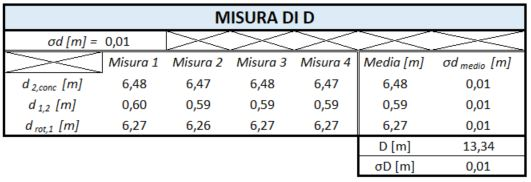
\includegraphics[width=0.5\linewidth]{RT_D.JPG}
    \caption{Misura del cammino ottico $D$}
    \label{RT_D}
\end{figure}

%RT_Apparato
\begin{figure}[h]
    \centering
    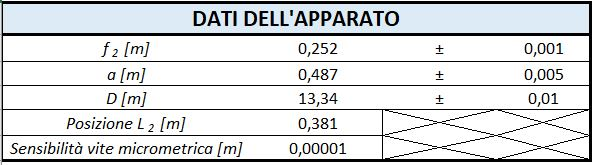
\includegraphics[width=0.6\linewidth]{RT_Apparato.JPG}
    \caption{Dati dell'apparato di Rossi e Tambini, comprensivi della focale $f_2$ della lente $L_2$ e della distanza tra $L_2$ e lo specchio rotante $a$}
    \label{RT_Apparato}
\end{figure}

%RT_DatiRaccolti
\begin{figure}[h!]
    \centering
    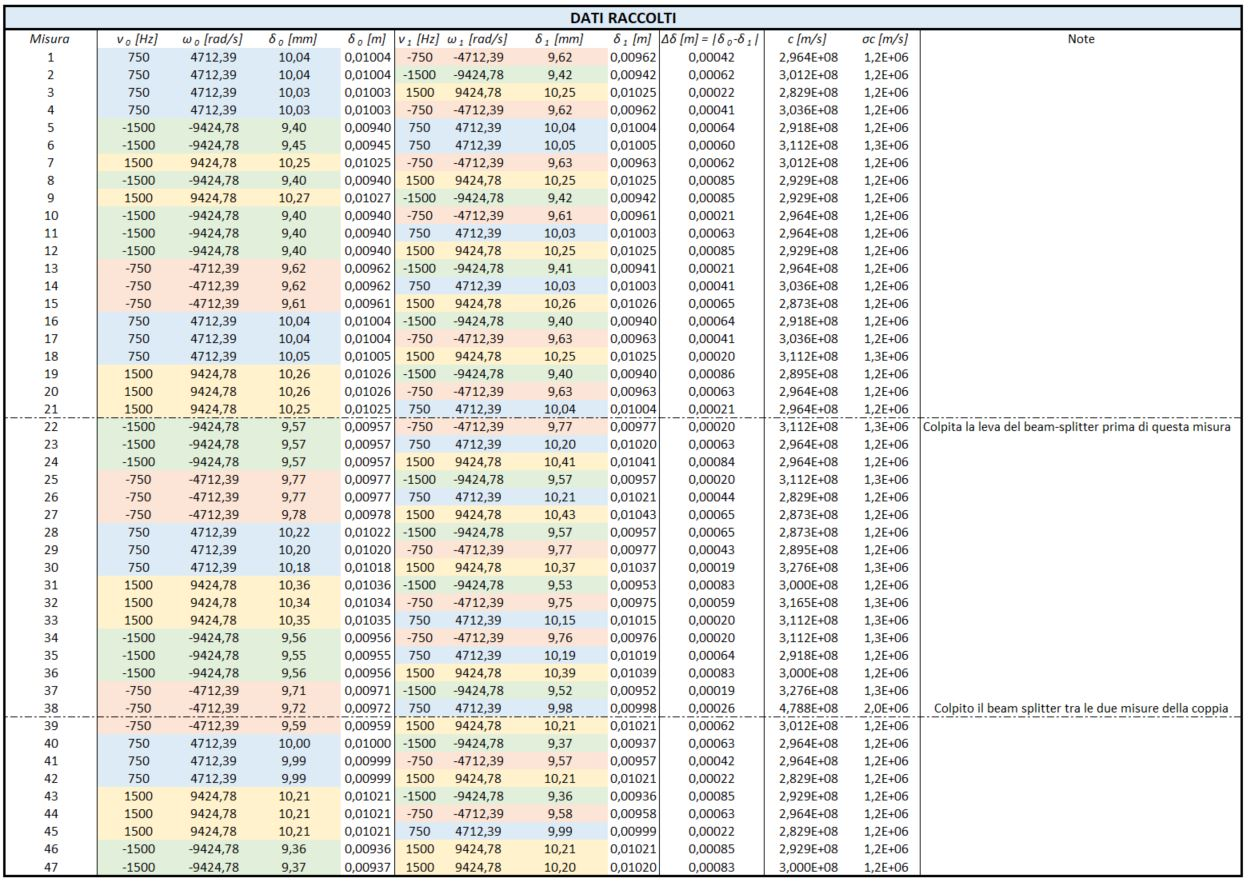
\includegraphics[width=1.02\linewidth]{RT_DatiRaccolti.JPG}
    \caption{Dati Raccolti da Rossi-Tambini. I valori di $\delta$ e $\delta_0$ misurati per una stessa frequenza di rotazione sono evidenziati col medesimo colore.}
    \label{RT_DatiRaccolti}
\end{figure}

%Tabelle_Coerenza
\begin{figure}[h]
    \centering
    \begin{subfigure}[h]{0.2\textwidth}
        \centering
        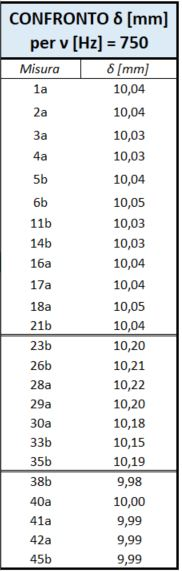
\includegraphics{Coerenza_T1.JPG}
        \caption{Misure raccolte per $\nu=750Hz$}
        \label{Tab_750}        
    \end{subfigure}
    \hfill
    \begin{subfigure}[h]{0.2\textwidth}
        \centering
        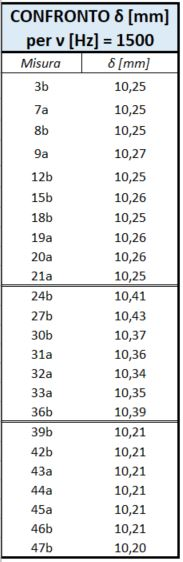
\includegraphics{Coerenza_T2.JPG}
        \caption{Misure raccolte per $\nu=1500Hz$}
        \label{Tab_1500}
    \end{subfigure}
    \hfill
    \begin{subfigure}[h]{0.2\linewidth}
        \centering
        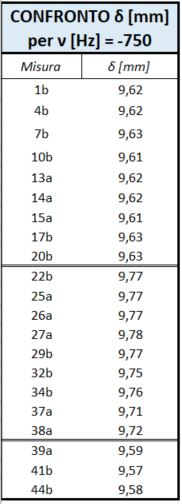
\includegraphics{Coerenza_T3.JPG}
        \caption{Misure raccolte per $\nu=-750Hz$}
        \label{Tab_-750}        
    \end{subfigure}
    \hfill
    \begin{subfigure}[h]{0.2\linewidth}
        \centering
        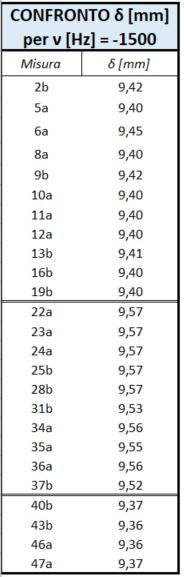
\includegraphics{Coerenza_T4.JPG}
        \caption{Misure raccolte per $\nu=-1500Hz$}
        \label{Tab_-1500}
    \end{subfigure}
        \caption{Dati raccolti in tabelle secondo la $\nu$ dello specchio rotante}
        \label{Tabs}
\end{figure}

%Coerenza_Grafici
\begin{figure}[h]
    \centering
    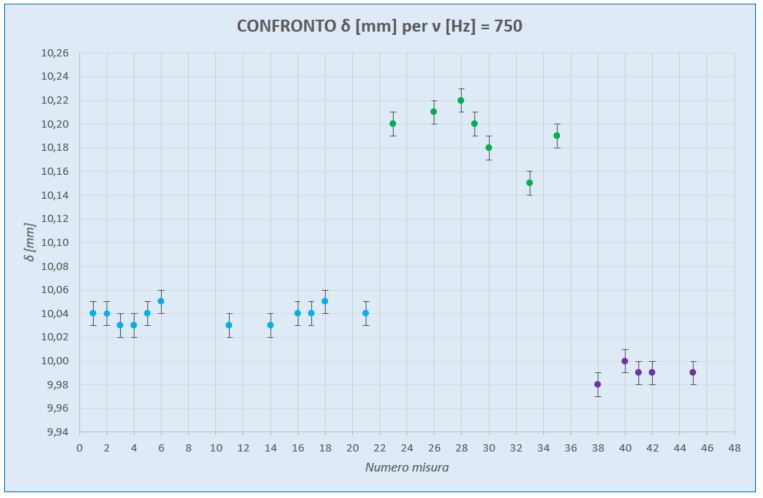
\includegraphics[width=0.8\textwidth]{Coerenza_G1.JPG}
    \caption{Grafico relativo a Figura (\ref{Tabs}\subref{Tab_750})}
    \label{Graf_750}
\end{figure}

\begin{figure}[h]
    \centering
    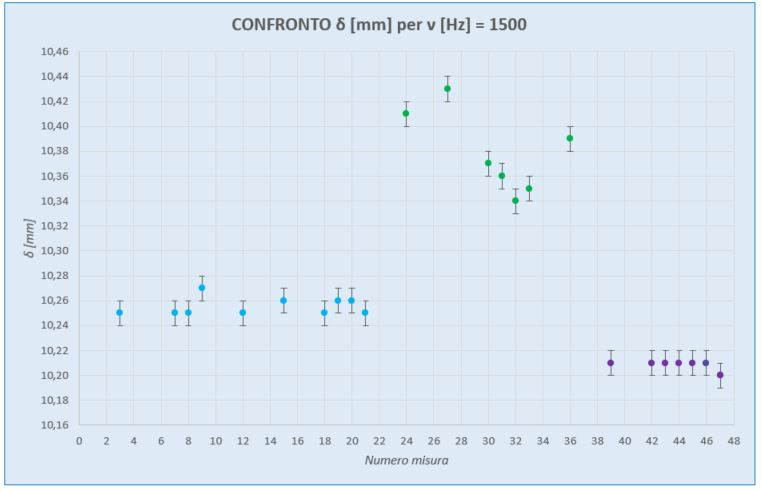
\includegraphics[width=0.8\textwidth]{Coerenza_G2.JPG}
    \caption{Grafico relativo a Figura (\ref{Tabs}\subref{Tab_1500})}
    \label{Graf_1500}
\end{figure}

\begin{figure}[h]
    \centering
    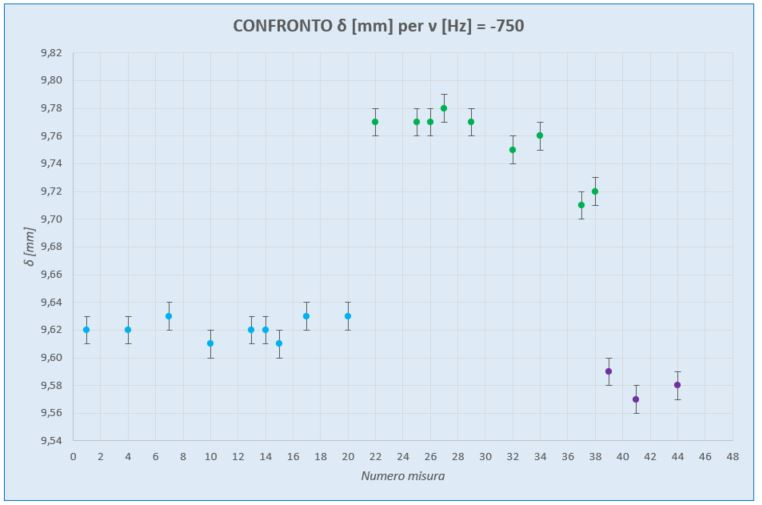
\includegraphics[width=0.8\textwidth]{Coerenza_G3.JPG}
    \caption{Grafico relativo a Figura (\ref{Tabs}\subref{Tab_-750})}
    \label{Graf_-750}
\end{figure}

\begin{figure}[h]
    \centering
    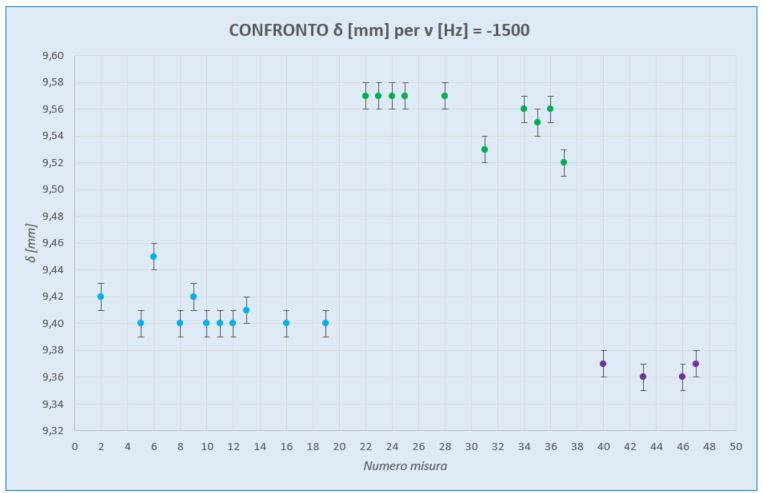
\includegraphics[width=0.8\textwidth]{Coerenza_G4.JPG}
    \caption{Grafico relativo a Figura (\ref{Tabs}\subref{Tab_-1500})}
    \label{Graf_-1500}
\end{figure}

%Coerenza_Gauss
\begin{figure}[h]
    \centering
    \begin{subfigure}{\linewidth}
        \centering
        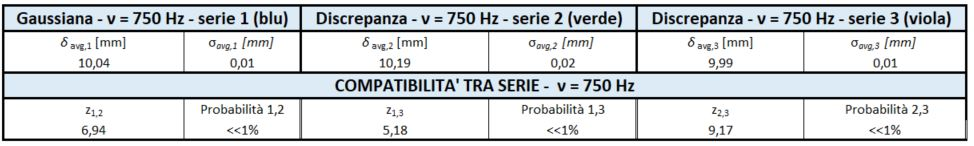
\includegraphics[width=\linewidth]{Coerenza_Gauss1.JPG}
        \caption{Distribuzione normale relativa a Figura (\ref{Tabs}\subref{Tab_750})}
        \label{Gauss_750}
    \end{subfigure}
    \newline
    \begin{subfigure}{\linewidth}
        \centering
        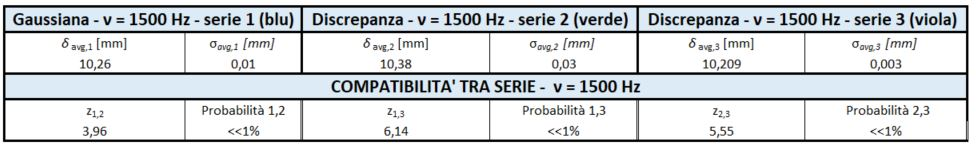
\includegraphics[width=\linewidth]{Coerenza_Gauss2.JPG}
        \caption{Distribuzione normale relativa a Figura (\ref{Tabs}\subref{Tab_1500})}
        \label{Gauss_1500}  
    \end{subfigure}
    \newline
    \begin{subfigure}{\linewidth}
        \centering
        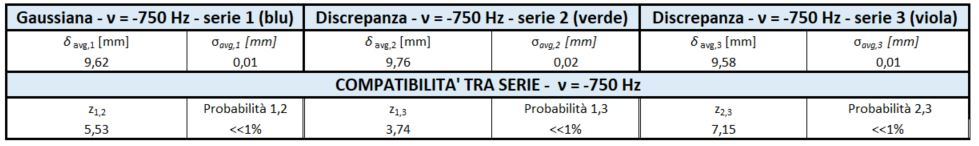
\includegraphics[width=\linewidth]{Coerenza_Gauss3.JPG}
        \caption{Distribuzione normale relativa a Figura (\ref{Tabs}\subref{Tab_-750})}
        \label{Gauss_-750}     
    \end{subfigure}
    \newline
    \begin{subfigure}{\linewidth}
        \centering
        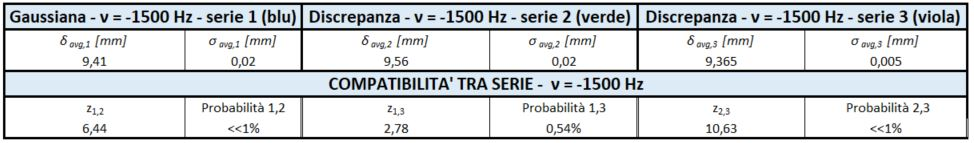
\includegraphics[width=\linewidth]{Coerenza_Gauss4.JPG}
        \caption{Distribuzione normale relativa a Figura (\ref{Tabs}\subref{Tab_-1500})}
        \label{Gauss_-1500}   
    \end{subfigure}
    \caption{Distribuzioni normali relative a Figura (\ref{Tabs})}
    \label{Gauss}
\end{figure}

%Rigetto misura 38
\begin{figure}[h]
    \centering
    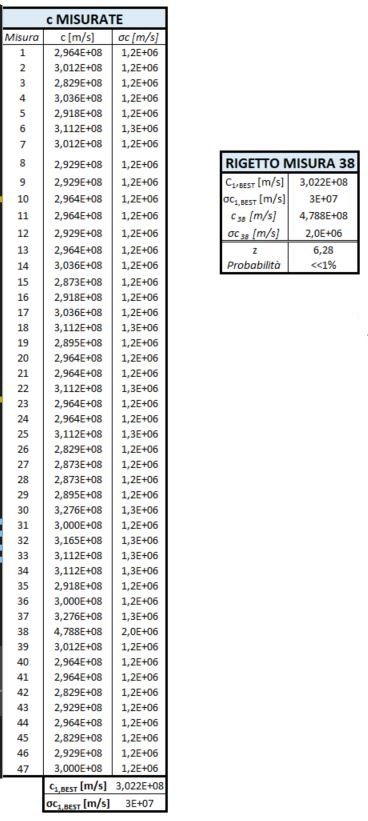
\includegraphics[width=0.6\linewidth]{Rigetto.JPG}
    \caption{Calcolo della migliore stima della velocità della luce basata sui valori raccolti da Rossi e Tambini $c_{1,BEST}$}
    \label{Rigetto}
\end{figure}
\FloatBarrier %creo una barriera invisibile per assicurarmi che la roba sia posizionata dove la dichiaro

\newpage
\subsection{Grafici e Tabelle - Ramella e Redaelli} \label{RAM}

% RAM_D
\begin{figure}[h!]
    \centering
    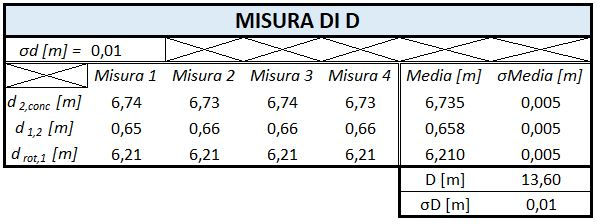
\includegraphics[width=0.55\linewidth]{RAM_D.JPG}
    \caption{Misura del cammino ottico $D$}
    \label{RAM_D}
\end{figure}

%RAM_Apparato
\begin{figure}[h!]
    \centering
    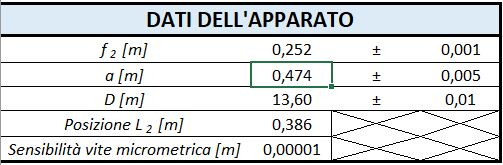
\includegraphics[width=0.5\linewidth]{RAM_Apparato.JPG}
    \caption{Dati dell'apparato di Ramella e Redaelli, comprensivi della focale $f_2$ della lente $L_2$ e della distanza tra $L_2$ e lo specchio rotante $a$}
    \label{RAM_Apparato}
\end{figure}

%DATI_CW
\begin{figure}[h!]
    \centering
    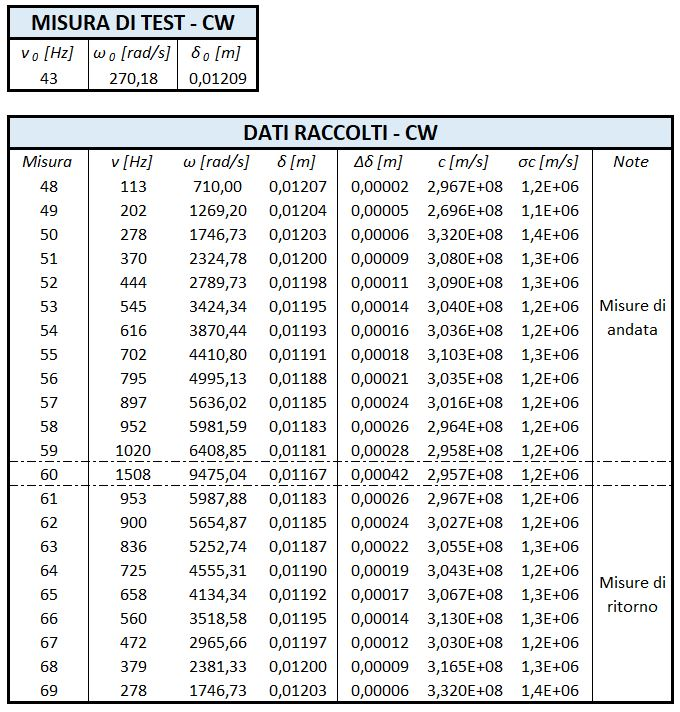
\includegraphics[width=0.6\linewidth]{RAM_CW.JPG}
    \caption{Dati raccolti per rotazioni in senso orario (CW)}
    \label{RAM_CW}
\end{figure}

%DATI_CCW
\begin{figure}[h]
    \centering
    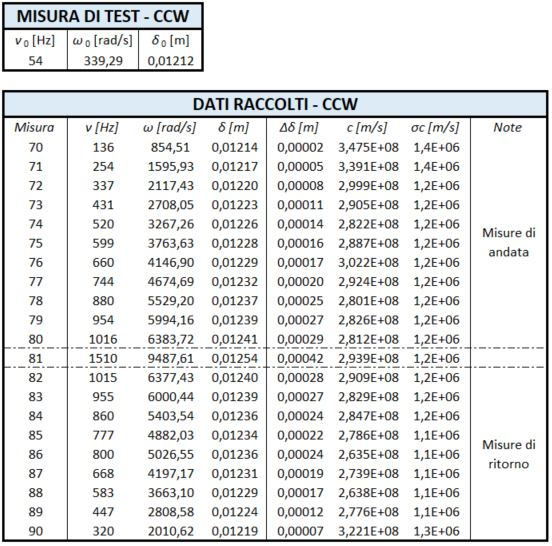
\includegraphics[width=0.6\linewidth]{RAM_CCW.JPG}
    \caption{Dati raccolti per rotazioni in senso antiorario (CCW)}
    \label{RAM_CCW}
\end{figure}

%DATI_TURBO
\begin{figure}[h]
    \centering
    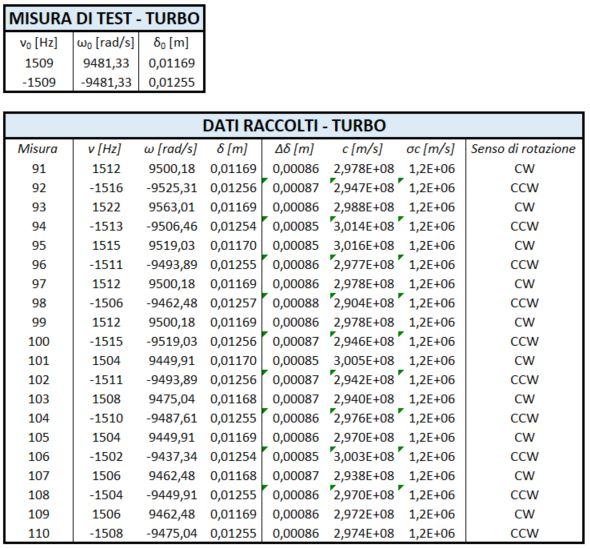
\includegraphics[width=0.6\linewidth]{RAM_TURBO.JPG}
    \caption{Dati raccolti per rotazioni in ambo i sensi alla massima velocità angolare}
    \label{RAM_TURBO}
\end{figure}

\FloatBarrier

\subsection{Grafici e Tabelle - Calcolo c} \label{C}

%Dati uniti
\begin{figure}[h!]
    \centering
    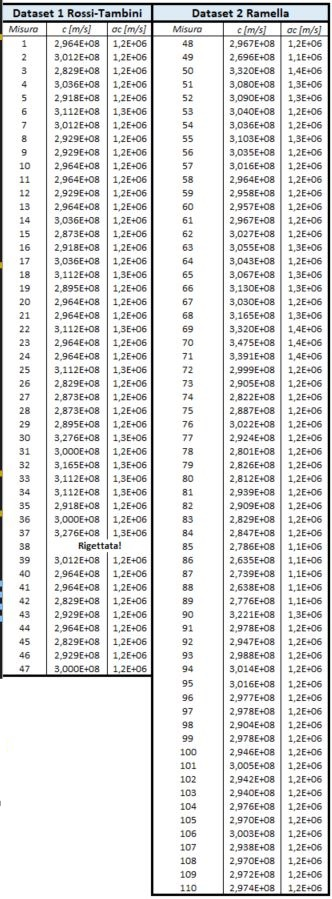
\includegraphics[width=0.47\linewidth]{Dati_Completi.JPG}
    \caption{Totalità dei dati raccolti, ad eccezione della misura 38, rigettata}
    \label{Dati_Completi}
\end{figure}

%Calcolo cbest
\begin{figure}[h]
    \centering
    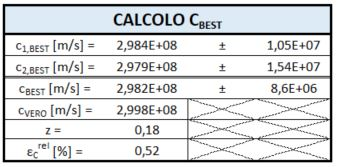
\includegraphics[width=0.5\linewidth]{Calcolo_cbest.JPG}
    \caption{Calcolo della miglior stima della velocità della luce $c_{BEST}$ basato sulla totalità dei dati raccolti}
    \label{Calcolo_cbest}
\end{figure}

%Grafico cbest
\begin{figure}[h]
    \centering
    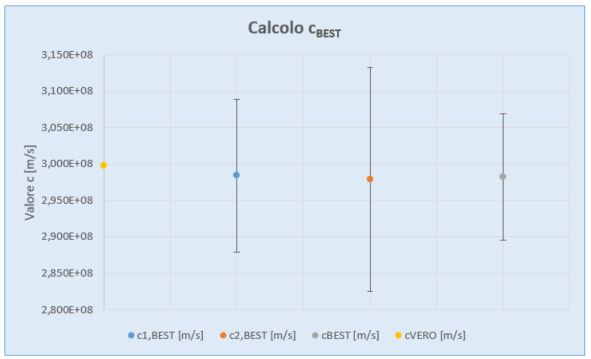
\includegraphics[width=0.8\linewidth]{Graf_cbest.JPG}
    \caption{Grafico dei valori $c_{1,BEST}$, $c_{2,BEST}$ e $c_{BEST}$ in relazione a $c_{vero}$}
    \label{Graf_cbest}
\end{figure}

\end{document}


% Å ^{\circ} \vspace{1mm} per spaziare verticalmente \begin{equation} e \end{equation} con dentro un \label e fuori un \ref per numerare e avere il riferimento alle
% equazioni È


